\task{Дорога до метро}

\noindent Рассмотрим клетчатую сетку, ее ребра и узлы. Путем между двумя узлами будем называть последовательность ребер, их соединяющую. Длину пути в разных случаях будем определять по-разному, однако стандартный способ~— понимать под длиной пути количество ребер в нем.

\ms Определим {\itshape $k$--окрестность} узла — это множество всех узлов, до которых от данного существует путь длиной не более чем $k$. На рисунке M1 изображены путь длины 3 и 3--окрестность центрального узла.

\begin{enumerate}

\item Длину пути можно ввести и по-другому. Давайте определим ее как сумму величин смещения пути по горизонтали и по вертикали.\linebreak Скажем, путь на рисунке M2 будет тогда иметь длину 5. Как будет выглядеть 4-окрестность фиксированного узла при так определеной длине?

\vspace{-0.3cm}
\begin{center}
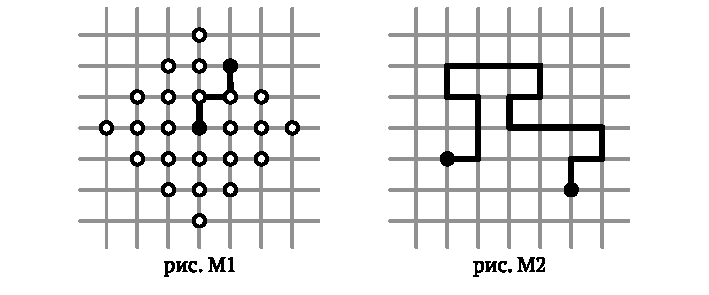
\includegraphics[width=10.5cm]{stats/2017/images/metro1.pdf}
\end{center} \vspace{-0.7cm}

\item А если мы определим длину пути как максимум; как минимум; как модуль разности величин смещения по горизонтали и по вертикали?

\item Рассмотрим два определения длины пути: стандартным способом и как в пункте 1. Понятно, что один путь может иметь разную длину в первом и во втором смысле. Докажите, тем не менее, что любая $k$--окрестность в смысле первой длины и в смысле второй длины выглядит одинаково.

\item Пусть длина пути определена стандартным образом. Пусть узел $B$ отстоит от узла $A$ на $m$ клеток вправо и на $n$ клеток вниз. Сколько кратчайших путей ведут из $A$ в $B$?

\end{enumerate}

\noindent Давайте теперь выберем из клетчатой сетки несколько узлов и некоторые ребра между ними. Назовем выбранное нами {\itshape городом}. Расположим в каких-то из узлов города {\itshape станции метро}. Расстоянием от узла внутри города до данной станции метро будем называть длину (в стандартном смысле) кратчайшего пути между ними, лежащего внутри города. На рисунке ниже изображены пример города, пара станций метро, а также кратчайшие пути от одного из узлов до станций.

\begin{center} \tikz{
	\filldraw [fill=softg, draw=softg] (0.3, -1.2) rectangle (0.7, 1.2); 
	\filldraw [fill=softg, draw=softg] (-0.2, -1.2) rectangle (0.7,-0.8); 
	\filldraw [fill=softg, draw=softg] (-0.7,-0.2) rectangle (0.7,0.2); 
	\filldraw [fill=softg, draw=softg] (-0.7,-0.2+0.5) rectangle (0.7,0.2+0.5); 
	\filldraw [fill=softg, draw=softg] (-0.7,-0.2) rectangle (-0.3,0.7); 

	\foreach \x in {-3,...,3} {
		\draw [color=hardg] (0.5 * \x cm, -2) -- (0.5 * \x cm, 2); 
		\draw [color=hardg] (-2, 0.5 * \x cm) -- (2, 0.5 * \x cm); 
	}

	\draw [very thick] (0,0)
		-- (-0.5,0)
		-- (-0.5,0.5)
		-- (0.5,0.5)
		-- (0.5,-1); 

	\foreach \x / \y in {0.5 / -1, 0 / 0}
		\filldraw[fill=black] (0.15cm + \x cm, \y cm) arc (0:360:0.15); 

	\begin{scope}[yshift=0.5 cm]
		\filldraw[fill=white,very thick]
			(0.1 cm,0.1 cm) -- ++(-0.2,0) -- ++(0,-0.2) -- ++(0.2,0) -- cycle; 
	\end{scope}
} \end{center}

\begin{enumerate} \setcounter{enumi}{4}

\item Для каждого узла в городе найдем ближайшую к нему станцию метро и расстояние до нее. Найдем в городе все узлы, в которых найденное расстояние достигает своего максимума. Теперь для каждого узла посчитаем сумму расстояний от него до всех станций метро и тоже найдем узлы, где эта сумма достигает максимального значения.

\smallskip\noindent Придумайте город и расстановку в нем станций метро такую, что множества узлов, где максимально кратчайшее расстояние, и узлов, где максимальна сумма расстояний, не пересекаются.

\item Докажите, что какой бы ни была расстановка станций метро в произвольном городе, максимальная сумма расстояний и максимальное среднее расстояние до станций всегда достигаются в одних и тех же узлах.

\item Для каждого узла в городе найдем самую далекую от него станцию метро и расстояние до нее. Найдем в городе все узлы, в которых найденное расстояние достигает своего максимума.

\smallskip\noindent Придумайте город и расстановку в нем станций метро такую, что три множества: узлов, где максимально кратчайшее расстояние; узлов, где максимальна сумма расстояний; узлов, где максимально наибольшее расстояние — не пересекаются.

\item Какие еще особенные узлы можно рассматривать в городе со станциями метро?  Предложите свои направления исследования и изучите их.

\end{enumerate}
